Formally define and draw an NFA that recognizes the language.

Let M be a NFA:
\begin{equation*}
  M = (K, \Sigma, \Delta, s, F)
\end{equation*}
where,
\begin{itemize}
  \item $K = \{ q_{0}, q_{1}, q_{2}, q_{3}, q_{4}, q_{5}, q_{6}, q_{7}, q_{8}, q_{9}, q_{10}, q_{11} \}$
  \item $\Sigma = \{ a, b \}$
  \item $s = q_0$, the initial state
  \item $F = \{ q_{11} \}$, final states
  \item The transition relation$\Delta = \left\{ \begin{aligned}
      &(q_0, a, q_1), (q_0, b, q_1), (q_0, e, q_1), (q_1, e, q_0), (q_1, a, q_2), (q_1, b, q_6),\\
      &(q_2, a, q_3), (q_3, a, q_4), (q_3, b, q_4), (q_3, e, q_4), (q_4, e, q_3), (q_4, b, q_5),\\
      &(q_5, b, q_{10}), (q_6, b, q_7), (q_7, a, q_8), (q_7, b, q_8), (q_7, e, q_8), (q_8, e, q_7),\\
      &(q_8, a, q_9), (q_9, a, q_{10}), (q_{10}, a, q_{11}), (q_{10}, b, q_{11}), (q_{10}, e, q_{11}), (q_{11}, e, q_{10}) \}
    \end{aligned} \right\}$
\end{itemize}

The NFA $M$:
\begin{figure}[ht!]
  \centering
  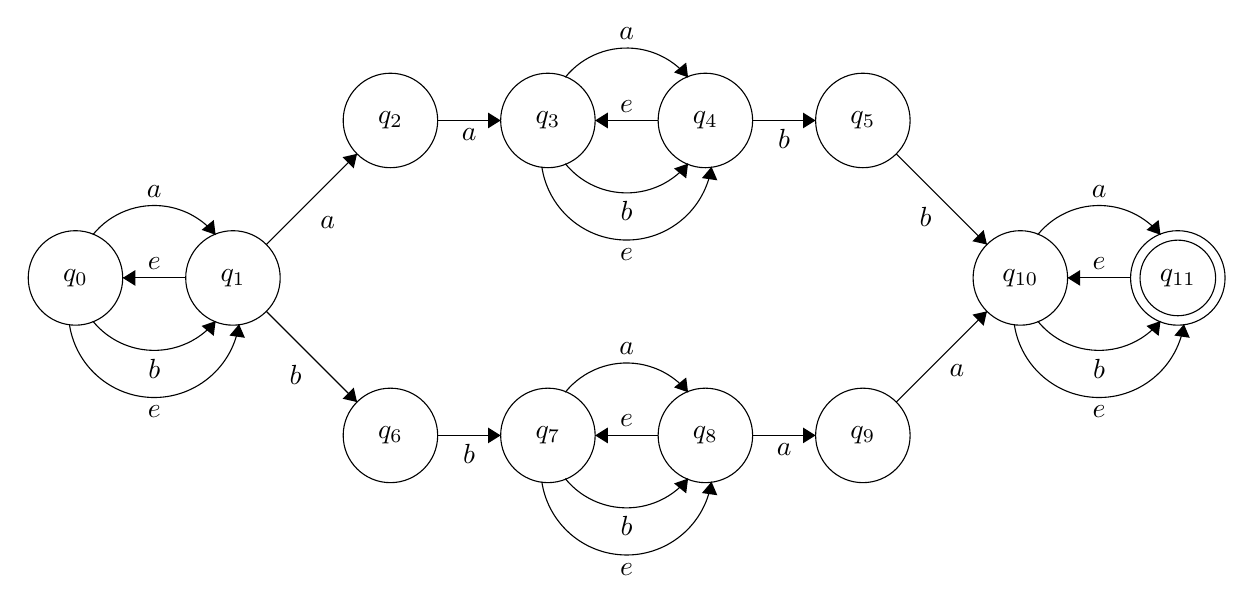
\begin{tikzpicture}[scale=0.2]
    \tikzstyle{every node}+=[inner sep=0pt]
    \draw [black] (3.3,-16.5) circle (3);
    \draw (3.3,-16.5) node {$q_0$};
    \draw [black] (13.3,-16.5) circle (3);
    \draw (13.3,-16.5) node {$q_1$};
    \draw [black] (23.3,-6.5) circle (3);
    \draw (23.3,-6.5) node {$q_2$};
    \draw [black] (33.3,-6.5) circle (3);
    \draw (33.3,-6.5) node {$q_3$};
    \draw [black] (43.3,-6.5) circle (3);
    \draw (43.3,-6.5) node {$q_4$};
    \draw [black] (53.3,-6.5) circle (3);
    \draw (53.3,-6.5) node {$q_5$};
    \draw [black] (23.3,-26.5) circle (3);
    \draw (23.3,-26.5) node {$q_6$};
    \draw [black] (33.3,-26.5) circle (3);
    \draw (33.3,-26.5) node {$q_7$};
    \draw [black] (43.3,-26.5) circle (3);
    \draw (43.3,-26.5) node {$q_8$};
    \draw [black] (53.3,-26.5) circle (3);
    \draw (53.3,-26.5) node {$q_9$};
    \draw [black] (63.3,-16.5) circle (3);
    \draw (63.3,-16.5) node {$q_{10}$};
    \draw [black] (73.3,-16.5) circle (3);
    \draw (73.3,-16.5) node {$q_{11}$};
    \draw [black] (73.3,-16.5) circle (2.4);
    \draw [black] (4.402,-13.758) arc (140.97764:39.02236:5.017);
    \fill [black] (12.2,-13.76) -- (12.08,-12.82) -- (11.31,-13.45);
    \draw (8.3,-11.4) node [above] {$a$};
    \draw [black] (12.198,-19.242) arc (-39.02236:-140.97764:5.017);
    \fill [black] (12.2,-19.24) -- (11.31,-19.55) -- (12.08,-20.18);
    \draw (8.3,-21.6) node [below] {$b$};
    \draw [black] (13.685,-19.437) arc (-8.31382:-171.68618:5.443);
    \fill [black] (13.69,-19.44) -- (13.08,-20.16) -- (14.06,-20.3);
    \draw (8.3,-24.59) node [below] {$e$};
    \draw [black] (15.42,-14.38) -- (21.18,-8.62);
    \fill [black] (21.18,-8.62) -- (20.26,-8.83) -- (20.97,-9.54);
    \draw (18.82,-12.98) node [right] {$a$};
    \draw [black] (10.3,-16.5) -- (6.3,-16.5);
    \fill [black] (6.3,-16.5) -- (7.1,-17) -- (7.1,-16);
    \draw (8.3,-16) node [above] {$e$};
    \draw [black] (26.3,-6.5) -- (30.3,-6.5);
    \fill [black] (30.3,-6.5) -- (29.5,-6) -- (29.5,-7);
    \draw (28.3,-7) node [below] {$a$};
    \draw [black] (34.402,-3.758) arc (140.97764:39.02236:5.017);
    \fill [black] (42.2,-3.76) -- (42.08,-2.82) -- (41.31,-3.45);
    \draw (38.3,-1.4) node [above] {$a$};
    \draw [black] (42.198,-9.242) arc (-39.02236:-140.97764:5.017);
    \fill [black] (42.2,-9.24) -- (41.31,-9.55) -- (42.08,-10.18);
    \draw (38.3,-11.6) node [below] {$b$};
    \draw [black] (43.685,-9.437) arc (-8.31382:-171.68618:5.443);
    \fill [black] (43.69,-9.44) -- (43.08,-10.16) -- (44.06,-10.3);
    \draw (38.3,-14.59) node [below] {$e$};
    \draw [black] (40.3,-6.5) -- (36.3,-6.5);
    \fill [black] (36.3,-6.5) -- (37.1,-7) -- (37.1,-6);
    \draw (38.3,-6) node [above] {$e$};
    \draw [black] (46.3,-6.5) -- (50.3,-6.5);
    \fill [black] (50.3,-6.5) -- (49.5,-6) -- (49.5,-7);
    \draw (48.3,-7) node [below] {$b$};
    \draw [black] (55.42,-8.62) -- (61.18,-14.38);
    \fill [black] (61.18,-14.38) -- (60.97,-13.46) -- (60.26,-14.17);
    \draw (57.28,-11.98) node [below] {$b$};
    \draw [black] (64.402,-13.758) arc (140.97764:39.02236:5.017);
    \fill [black] (72.2,-13.76) -- (72.08,-12.82) -- (71.31,-13.45);
    \draw (68.3,-11.4) node [above] {$a$};
    \draw [black] (72.198,-19.242) arc (-39.02236:-140.97764:5.017);
    \fill [black] (72.2,-19.24) -- (71.31,-19.55) -- (72.08,-20.18);
    \draw (68.3,-21.6) node [below] {$b$};
    \draw [black] (73.685,-19.437) arc (-8.31382:-171.68618:5.443);
    \fill [black] (73.69,-19.44) -- (73.08,-20.16) -- (74.06,-20.3);
    \draw (68.3,-24.59) node [below] {$e$};
    \draw [black] (70.3,-16.5) -- (66.3,-16.5);
    \fill [black] (66.3,-16.5) -- (67.1,-17) -- (67.1,-16);
    \draw (68.3,-16) node [above] {$e$};
    \draw [black] (15.42,-18.62) -- (21.18,-24.38);
    \fill [black] (21.18,-24.38) -- (20.97,-23.46) -- (20.26,-24.17);
    \draw (17.28,-21.98) node [below] {$b$};
    \draw [black] (26.3,-26.5) -- (30.3,-26.5);
    \fill [black] (30.3,-26.5) -- (29.5,-26) -- (29.5,-27);
    \draw (28.3,-27) node [below] {$b$};
    \draw [black] (34.402,-23.758) arc (140.97764:39.02236:5.017);
    \fill [black] (42.2,-23.76) -- (42.08,-22.82) -- (41.31,-23.45);
    \draw (38.3,-21.4) node [above] {$a$};
    \draw [black] (42.198,-29.242) arc (-39.02236:-140.97764:5.017);
    \fill [black] (42.2,-29.24) -- (41.31,-29.55) -- (42.08,-30.18);
    \draw (38.3,-31.6) node [below] {$b$};
    \draw [black] (43.685,-29.437) arc (-8.31382:-171.68618:5.443);
    \fill [black] (43.69,-29.44) -- (43.08,-30.16) -- (44.06,-30.3);
    \draw (38.3,-34.59) node [below] {$e$};
    \draw [black] (40.3,-26.5) -- (36.3,-26.5);
    \fill [black] (36.3,-26.5) -- (37.1,-27) -- (37.1,-26);
    \draw (38.3,-26) node [above] {$e$};
    \draw [black] (46.3,-26.5) -- (50.3,-26.5);
    \fill [black] (50.3,-26.5) -- (49.5,-26) -- (49.5,-27);
    \draw (48.3,-27) node [below] {$a$};
    \draw [black] (55.42,-24.38) -- (61.18,-18.62);
    \fill [black] (61.18,-18.62) -- (60.26,-18.83) -- (60.97,-19.54);
    \draw (59.27,-21.98) node [below] {$a$};
  \end{tikzpicture}
  \caption{$M$}  
\end{figure}
